\ifthenelse{\boolean{pcppapermadweb}}{
    \pagestyle{plain}
\title{Five Word Password Composition Policy}

\author{\IEEEauthorblockN{Sirvan Almasi}
	\IEEEauthorblockA{Imperial College London\\
		sirvan.almasi17@imperial.ac.uk},
	\and
	\IEEEauthorblockN{William J.\,Knottenbelt}
	\IEEEauthorblockA{Imperial College London\\
        w.knottenbelt@imperial.ac.uk}
}


\IEEEoverridecommandlockouts
\makeatletter\def\@IEEEpubidpullup{6.5\baselineskip}\makeatother
\IEEEpubid{\parbox{\columnwidth}{
    {\fontsize{7.5}{7.5}\selectfont Workshop on Measurements, Attacks, and Defenses for the Web (MADWeb) 2025\\
    28 February 2025, San Diego, CA, USA\\
    ISBN 979-8-9894372-9-0\\
    https://dx.doi.org/10.14722/madweb.2025.23020\\
    www.ndss-symposium.org}
}
\hspace{\columnsep}\makebox[\columnwidth]{}}


\maketitle

\begin{abstract}
Password composition policies (PCPs) are critical security rules that govern how users create passwords for online authentication. Despite passwords remaining the primary authentication method online, there is significant disagreement among experts, regulatory bodies, and researchers about what constitutes effective password policies. This lack of consensus has led to high variance in PCP implementations across websites, leaving both developers and users uncertain. Current approaches lack a theoretical foundation for evaluating and comparing different password composition policies. We show that a structure-based policy, such as the three-random words recommended by UK's National Cyber Security Centre (NCSC), can improve password security. We demonstrate this using an empirical evaluation of labelled password datasets and a new theoretical framework. Using these methods we demonstrate the feasibility and security of multi-word password policy and extend the NCSC's recommendation to five words to account for non-uniform word selection. These findings provide an evidence-based framework for password policy development and suggest that current web authentication systems should adjust their minimum word requirements upward while maintaining usability.
\end{abstract}

\section{Introduction}

The lack of consensus on password composition policy (PCP) and the lack of adoption of best practices on the web~\cite{alroomi_measuring_2023, lomchan_comparison_2023, lim_evaluating_2023, maoneke_password_2019, furnell_assessing_2011, woo_survey_2018, lee_password_2022, gerlitz_please_2021} suggests that our knowledge on password security is not yet complete. Although passwords remain the main method of authentication, experts and regulatory bodies disagree fundamentally about what makes a good password policy. State agencies recommend one set of rules, while professional organisations suggest another, and academic researchers advocate for yet different approaches. This lack of consensus reveals a troubling gap in our understanding of password security. What password composition rules should web developers implement to best protect their users?

National organisations such as NIST~(US)~\cite{nist2024} and NCSC~(UK)~\cite{ncsc2024} provide similar guidance on PCP, UK's NCSC additionally recommends minimum of three word password structure. This paper is most interested in structure related policies to enhance user secret security--should a system or web admin recommend such three word password structure policies? In this paper, we develop a model that allows us to reason analytically about PCPs. Using this, we tackle the PCP recommended by the UK's NCSC (minimum of three random words). We present a novel theoretical framework for analysing password composition policies, bridging the gap between security requirements and user behaviour.

The gap between research and practice compounds the inconsistency in the PCP recommendation. Consider Dropbox, which developed \zxcvbn Password Strength Meter (PSM). Despite creating this tool, which has 14.7K Github stars and has been validated by independent research~\cite{wang_no_2023}, Dropbox's own web authentication policy contradicts current best practices. Their website requires passwords with a minimum of eight characters, one letter, one digit, and one symbol. Even more concerning, they do not appear to use their own PSM. \zxcvbn has some weaknesses; it awards its maximum score of 4/4 to \password{girlsruledaworld} and a strong 3/4 to \password{asdf1fdsa1}---passwords that we would consider vulnerable as they are common phrases or sequences.

\textbf{\textsc{Threat Scenario.}} We assume that some users will choose memorable passwords, eschewing password managers or WebAuthn alternatives. Although password managers offer stronger security, our model addresses the reality that many users, from a broad population, will rely on human-generated passwords. Passwords are also useful in offline and air-gapped systems too where out-of-band systems are limited. Therefore, system and web admins have to consider such scenarios. We therefore analyse password security against the most challenging threat model: an offline attack where adversaries can make unlimited guessing attempts without rate limiting.
\vspace*{0.25cm}

\textbf{\textsc{Our Contributions are as Follows:}}
\begin{itemize}
    \item Empirical validation of a structure-based password policy in addition to existing policies. This provides quantitative support for existing password composition recommendations, particularly the NCSC's three-word policy
    \item A formal mathematical model describing the recommended number of words to mitigate user behaviours such as choosing words from a non-uniform distribution.
\end{itemize}

\vspace*{0.25cm}

This work addresses core areas of web security, and our results provide actionable insights for improving password policies across web platforms while maintaining usability. Our findings and insights provide immediate applications for system and web admins. Our work also provides a theoretical and reasoning basis for future password composition policy development and research.

\newpage
\section{Background}
\label{sec::chp4::background}

\textbf{\textsc{Password\;Strength.}}\;This metric measures the difficulty of guessing or cracking a password. However, there is no consensus on how to quantify such difficulty. Some experts use dictionary-based methods, while others rely on probabilistic deep-learning based approaches. Nonetheless, certain lower-bound measures are widely accepted, such as the minimum number of characters required to prevent brute-force attacks.

Shannon's entropy (Eq. \ref{eq:entropy}) quantifies the uncertainty or information content associated with a random variable. \begin{equation}\label{eq:entropy}
H(X) = -\sum_{x\in\mathcal{X}}^{} p(x) \log p(x)
\end{equation} In the context of password strength, it measures how unpredictable or "random" a password is. The higher the entropy, the more difficult the password is to guess, making it stronger. This metric estimates the minimum number of bits required to encode the password. However, the entropy measure for passwords is often given in the form of $\log_2(R^L)$, where $R$ represents the total number of characters in the character sets used in the password, and $L$ is the length of the password.

The limitation of $\log_2(R^L)$ is that it assumes all $R$ characters are equally likely, disregarding the dependency between characters in human-chosen passwords. This approach oversimplifies, as passwords like \password{8zm!U6gNL\%} and \password{p4\$sW0rd1!} are calculated to have the same entropy. However, such an assumption is unrealistic, as the latter password is essentially the word \textit{password} with predictable transformations.

\textbf{\textsc{Password Composition Policies (PCP).}}\: PCP is set of rules, often in natural language, that only allows the user to sample from a password space that is assumed to be resistant to guessing attacks. The \textit{National Cyber Security Centre (NCSC)}~\cite{ncsc2024} in the UK and the \textit{National Institute of Standards and Technology (NIST)}~\cite{nist2024} in the USA are leading authorities in cyber-security. Their recommendations, particularly on password policies, should serve as standards or benchmarks in the field. Specifically, the NCSC advocates for the use of three random words~\cite{McCormackthreerandom} and advises against mandatory password complexity requirements~\cite{password_policy_ncsc}. This approach, detailed in~\cite{Kate_2021}, is based on the principle that a sequence of three random words is both easier for users to remember and sufficiently complex to deter unauthorised access, striking a balance between security and user convenience. This three word and structure-based PCP is conditioned on the following:

\begin{itemize}[itemsep=0pt, parsep=0pt, leftmargin=11pt]
    \item \textsc{\textbf{Length}}. To satisfy the minimum length requirements.
    \item \textsc{\textbf{Impact}}. Easy to adopt and understand.
    \item \textsc{\textbf{Novelty}}. Unlikely to find it in a breached database.
    \item \textsc{\textbf{Usability}}. More likely to be remembered.
\end{itemize}
\label{jmp::chp4::ncsc-pcp}

NIST's \cite{Grassi_Garcia_Fenton_2020} PCP is as follows. Passwords should have a minimum length of 8 characters, but systems should support more than 64 characters. It is advised to compare the selected password against prior breach data, dictionary entries, and repetitive patterns. Context-specific terms should also be considered. Additionally, users should be aided with strength meters to gauge password robustness. While rate limiting should be enforced during authentication attempts, use of specific composition rules is discouraged.
OWASP \cite{owasp_owasp_2024} follows the recommendations set by NIST.

\textbf{\textsc{passwordNinja Dataset \cite{almasi2024passwordninja}}} is a human and machine labelled datasets that has decomposed password strings into its finer constituents. For example, the password \password{0rwell1984} would be structured as follows.
\[
\begin{aligned}
& \underbrace{\text{\password{0rwell}}}_{\text{word }(w)} \underbrace{\text{\password{1984}}}_{\text{date}} \\[10pt]
\end{aligned}
\vspace*{-0.3cm}
\]
The \fun{passwordNinja}~\cite{almasi2024passwordninja} dataset is composed of a complete \hmail and \lizardsquad breached passwords from 2009 and 2015 respectively. The \hmail dataset, which leaked in 2009~\cite{johnson_hotmail_2009}, comprises \num{8929} records of passwords. Public sources indicate that these passwords were procured through phishing. Abundant evidence within the dataset supports this claim. For instance, we observe numerous passwords with inverted capitalisation and similar passwords that contain typos, suggesting that users might have unintentionally activated \texttt{CAPS\;LOCK}. The \lizardsquadnocite dataset contains \num{11808} records.
}{}
\vspace*{-0.7cm}
\section{Password\;Composition\;Policy}
\vspace*{-0.4cm}
\label{sec::chp4::pcp}
\begin{figure*}[ht]
    \centering
    \begin{subfigure}[b]{0.45\linewidth}
        \centering
        \scalebox{1}{\input{figs/why_passwords/word_freq_loglog}}
        \caption{Unique Words}
        \label{fig:word_freq_loglog}
    \end{subfigure}
    \hspace{0.5cm} % Space between the two figures
    \begin{subfigure}[b]{0.45\linewidth}
        \centering
        \scalebox{1}{\input{figs/why_passwords/structure_loglog}}
        \caption{Structures}
        \label{fig:structure_loglog}
    \end{subfigure}
    \caption{Charts showing the log-log plot of word and structure against their respective rank for the \hmail dataset. Words are from extracted unique passwords. The distribution of both words and structure exhibit a power law similar to Zipf's law.}
    \label{fig:log-log-charts}
    %\vspace{-1.5em} % Adjust the negative value to reduce the gap
\end{figure*}

\begin{table*}[h]
    \centering
    %\footnotesize
    \scriptsize
    
    \caption{The table presents the top 25 labelled password structures from the passwordNinja \cite{almasi2024passwordninja} dataset, accounting for 5\,032 (69.5\%) of the labelled dataset. Hashcat \cite{steube_hashcat_2023} benchmarks indicate the performance of consumer hardware in a hybrid attack. The dictionary size for $\bm{w}$ (words) and $\bm{n}$ (numbers) is set at $5\times 10^5$. \zxcvbn serves as a password strength meter, with scores ranging from 0 to 4, and guess estimates are log based.}
    \label{table:structures}
    \setlength\tabcolsep{1pt} % default value: 6pt
    {\renewcommand{\arraystretch}{0.3}% for the vertical padding
    \begin{tabular}{rllc|cccc|cc}
    % \toprule
     & & \multicolumn{2}{c}{Frequency}  & \multicolumn{4}{c}{Hashcat using Nvidia RTX 4090} & \multicolumn{2} {c}{\zxcvbnnocite Mean} \\\cmidrule{3-4} \cmidrule{5-10}
    \textbf{Structure} & \textbf{$log$ perm'} & \textbf{Count} & \textbf{\%} & \textbf{MD5} & \textbf{PBKDF2-sha256} & \textbf{scrypt} & \textbf{bcrypt-sha512} & \textbf{Score} & \textbf{Guesses} \\
    \midrule
w & \DrawLengthBarThick{4.7} & \DrawLengthBarThick{15.2} 1520 & 21.0 & $\sim0$ & 0.1 s & 1 min & 4 min & 1.3 & 5.36 \\
n & \DrawLengthBarThick{4.7} & \DrawLengthBarThick{8.11} 811 & 11.2 & $\sim0$ & 0.1 s & 1 min & 4 min & 1.0 & 4.72 \\
nd & \DrawLengthBarThick{5.6} & \DrawLengthBarThick{0.58} 58 & 0.8 & $\sim0$ & 0.6 s & 12 min & 42 min & 1.4 & 5.68 \\
wd & \DrawLengthBarThick{5.6} & \DrawLengthBarThick{0.91} 91 & 1.3 & $\sim0$ & 0.6 s & 12 min & 42 min & 1.5 & 5.97 \\
nl & \DrawLengthBarThick{5.9} & \DrawLengthBarThick{0.33} 33 & 0.5 & $\sim0$ & 1.5 s & 30 min & 2 h & 1.2 & 5.09 \\
wdd & \DrawLengthBarThick{6.4} & \DrawLengthBarThick{2.94} 294 & 4.1 & $\sim0$ & 5.6 s & 2 h & 7 h & 1.8 & 6.69 \\
ndd & \DrawLengthBarThick{6.4} & \DrawLengthBarThick{2.21} 221 & 3.1 & $\sim0$ & 5.6 s & 2 h & 7 h & 1.6 & 6.33 \\
nddd & \DrawLengthBarThick{7.2} & \DrawLengthBarThick{0.71} 71 & 1.0 & $\sim0$ & 56.4 s & 19 h & 3 day & 1.7 & 6.37 \\
wddd & \DrawLengthBarThick{7.2} & \DrawLengthBarThick{0.91} 91 & 1.3 & $\sim0$ & 56.4 s & 19 h & 3 day & 1.9 & 6.84 \\
wsdd & \DrawLengthBarThick{7.6} & \DrawLengthBarThick{0.29} 29 & 0.4 & $\sim0$ & 3 min & 3 day & 9 day & 2.0 & 7.28 \\
ddddw & \DrawLengthBarThick{8.1} & \DrawLengthBarThick{0.35} 35 & 0.5 & $\sim0$ & 9 min & 8 day & 29 day & 2.4 & 7.95 \\
wdddd & \DrawLengthBarThick{8.1} & \DrawLengthBarThick{1.74} 174 & 2.4 & $\sim0$ & 9 min & 8 day & 29 day & 2.3 & 7.59 \\
ndddd & \DrawLengthBarThick{8.1} & \DrawLengthBarThick{2.05} 205 & 2.8 & $\sim0$ & 9 min & 8 day & 29 day & 2.0 & 6.90 \\
nn & \DrawLengthBarThick{9.5} & \DrawLengthBarThick{3.76} 376 & 5.2 & 1.5 s & 8 h & 1 yr & 4 yr & 2.0 & 6.91 \\
ww & \DrawLengthBarThick{9.5} & \DrawLengthBarThick{4.57} 457 & 6.3 & 1.5 s & 8 h & 1 yr & 4 yr & 2.0 & 7.04 \\
nw & \DrawLengthBarThick{9.5} & \DrawLengthBarThick{0.3} 30 & 0.4 & 1.5 s & 8 h & 1 yr & 4 yr & 2.2 & 7.51 \\
ndddddd & \DrawLengthBarThick{9.7} & \DrawLengthBarThick{0.51} 51 & 0.7 & 3.0 s & 16 h & 2 yr & 8 yr & 2.5 & 8.05 \\
wdddddd & \DrawLengthBarThick{9.7} & \DrawLengthBarThick{0.33} 33 & 0.5 & 3.0 s & 16 h & 2 yr & 8 yr & 2.8 & 8.84 \\
wwdd & \DrawLengthBarThick{11.1} & \DrawLengthBarThick{0.58} 58 & 0.8 & 3 min & 33 day & 111 yr & 402 yr & 2.9 & 8.97 \\
nndd & \DrawLengthBarThick{11.1} & \DrawLengthBarThick{0.38} 38 & 0.5 & 3 min & 33 day & 111 yr & 402 yr & 3.2 & 9.62 \\
wwdddd & \DrawLengthBarThick{12.8} & \DrawLengthBarThick{0.33} 33 & 0.5 & 4 h & 9 yr & $1.11 \times 10^{4}$ yr & $4.02 \times 10^{4}$ yr & 3.3 & 9.81 \\
nwn & \DrawLengthBarThick{14.2} & \DrawLengthBarThick{0.41} 41 & 0.6 & 9 day & 447 yr & $5.56 \times 10^{5}$ yr & $2.01 \times 10^{6}$ yr & 3.0 & 8.88 \\
www & \DrawLengthBarThick{14.2} & \DrawLengthBarThick{1.65} 165 & 2.3 & 9 day & 447 yr & $5.56 \times 10^{5}$ yr & $2.01 \times 10^{6}$ yr & 3.0 & 9.26 \\
nww & \DrawLengthBarThick{14.2} & \DrawLengthBarThick{0.35} 35 & 0.5 & 9 day & 447 yr & $5.56 \times 10^{5}$ yr & $2.01 \times 10^{6}$ yr & 2.7 & 8.18 \\
nnn & \DrawLengthBarThick{14.2} & \DrawLengthBarThick{0.27} 27 & 0.4 & 9 day & 447 yr & $5.56 \times 10^{5}$ yr & $2.01 \times 10^{6}$ yr & 3.3 & 9.95 \\
wwww & \DrawLengthBarThick{15.3} & \DrawLengthBarThick{0.55} 55 & 0.8 & 171 day & $8.70 \times 10^{3}$ yr & $1.08 \times 10^{7}$ yr & $3.91 \times 10^{7}$ yr & 3.5 & 11.24 \\
\bottomrule
    \end{tabular}
    } %% vertical padding
\end{table*}
\ifthenelse{\boolean{pcppapermadweb}}{}{
\begin{table*}[!ht]
    \centering
    %\footnotesize
    \scriptsize
    \caption{The table presents the top 25 labelled password structures from the Lizard-Squad dataset. Hashcat \cite{steube_hashcat_2023} benchmarks indicate the performance of consumer hardware in a hybrid attack. The dictionary size for $\bm{w}$ (words) and $\bm{n}$ (numbers) is set at $5\times 10^5$. \zxcvbn serves as a password strength meter, with scores ranging from 0 to 4, and guess estimates are log based.}
    \label{table:ls-structures}
    \setlength\tabcolsep{1pt} % default value: 6pt
    {\renewcommand{\arraystretch}{0.3}% for the vertical padding
    \begin{tabular}{rllc|cccc|cc}
    % \toprule
     & & \multicolumn{2}{c}{Frequency}  & \multicolumn{4}{c}{Hashcat using Nvidia RTX 4090} & \multicolumn{2} {c}{\zxcvbnnocite Mean} \\\cmidrule{3-4} \cmidrule{5-10}
    \textbf{Structure} & \textbf{$log$ perm'} & \textbf{Count} & \textbf{\%} & \textbf{MD5} & \textbf{PBKDF2-sha256} & \textbf{scrypt} & \textbf{bcrypt-sha512} & \textbf{Score} & \textbf{Guesses} \\
    \midrule
w & \DrawLengthBarThick{4.7} & \DrawLengthBarThick{5.94} 594 & 5.5 & $\sim0$ & 0.1 s & 1 min & 4 min & 0.9 & 4.24 \\
n & \DrawLengthBarThick{4.7} & \DrawLengthBarThick{1.89} 189 & 1.7 & $\sim0$ & 0.1 s & 1 min & 4 min & 0.8 & 4.13 \\
wd & \DrawLengthBarThick{5.6} & \DrawLengthBarThick{2.54} 254 & 2.3 & $\sim0$ & 0.6 s & 12 min & 42 min & 1.2 & 5.06 \\
nd & \DrawLengthBarThick{5.6} & \DrawLengthBarThick{1.35} 135 & 1.2 & $\sim0$ & 0.6 s & 12 min & 42 min & 1.5 & 5.71 \\
wdd & \DrawLengthBarThick{6.4} & \DrawLengthBarThick{6.67} 667 & 6.1 & $\sim0$ & 5.6 s & 2 h & 7 h & 1.4 & 5.64 \\
ndd & \DrawLengthBarThick{6.4} & \DrawLengthBarThick{4.57} 457 & 4.2 & $\sim0$ & 5.6 s & 2 h & 7 h & 1.4 & 5.85 \\
wddd & \DrawLengthBarThick{7.2} & \DrawLengthBarThick{7.36} 736 & 6.8 & $\sim0$ & 56.4 s & 19 h & 3 day & 1.6 & 6.10 \\
nddd & \DrawLengthBarThick{7.2} & \DrawLengthBarThick{4.09} 409 & 3.8 & $\sim0$ & 56.4 s & 19 h & 3 day & 1.6 & 6.04 \\
wdddd & \DrawLengthBarThick{8.1} & \DrawLengthBarThick{4.65} 465 & 4.3 & $\sim0$ & 9 min & 8 day & 29 day & 1.7 & 6.41 \\
ndddd & \DrawLengthBarThick{8.1} & \DrawLengthBarThick{3.59} 359 & 3.3 & $\sim0$ & 9 min & 8 day & 29 day & 1.7 & 6.18 \\
nddddd & \DrawLengthBarThick{8.9} & \DrawLengthBarThick{0.58} 58 & 0.5 & 0.3 s & 2 h & 81 day & 293 day & 1.8 & 6.51 \\
wddddd & \DrawLengthBarThick{8.9} & \DrawLengthBarThick{0.84} 84 & 0.8 & 0.3 s & 2 h & 81 day & 293 day & 2.0 & 6.89 \\
nn & \DrawLengthBarThick{9.5} & \DrawLengthBarThick{1.39} 139 & 1.3 & 1.5 s & 8 h & 1 yr & 4 yr & 1.6 & 6.03 \\
nw & \DrawLengthBarThick{9.5} & \DrawLengthBarThick{0.26} 26 & 0.2 & 1.5 s & 8 h & 1 yr & 4 yr & 1.8 & 6.42 \\
ww & \DrawLengthBarThick{9.5} & \DrawLengthBarThick{6.66} 666 & 6.1 & 1.5 s & 8 h & 1 yr & 4 yr & 1.5 & 5.84 \\
ndddddd & \DrawLengthBarThick{9.7} & \DrawLengthBarThick{0.51} 51 & 0.5 & 3.0 s & 16 h & 2 yr & 8 yr & 2.3 & 7.24 \\
wdddddd & \DrawLengthBarThick{9.7} & \DrawLengthBarThick{0.52} 52 & 0.5 & 3.0 s & 16 h & 2 yr & 8 yr & 1.9 & 6.92 \\
nnd & \DrawLengthBarThick{10.3} & \DrawLengthBarThick{0.73} 73 & 0.7 & 15.2 s & 3 day & 11 yr & 40 yr & 2.4 & 7.82 \\
wwd & \DrawLengthBarThick{10.3} & \DrawLengthBarThick{2.31} 231 & 2.1 & 15.2 s & 3 day & 11 yr & 40 yr & 2.1 & 7.18 \\
wwdd & \DrawLengthBarThick{11.1} & \DrawLengthBarThick{3.07} 307 & 2.8 & 3 min & 33 day & 111 yr & 402 yr & 2.4 & 7.61 \\
nndd & \DrawLengthBarThick{11.1} & \DrawLengthBarThick{0.86} 86 & 0.8 & 3 min & 33 day & 111 yr & 402 yr & 2.8 & 8.64 \\
wwddd & \DrawLengthBarThick{12.0} & \DrawLengthBarThick{2.33} 233 & 2.1 & 25 min & 326 day & $1.11 \times 10^{3}$ yr & $4.02 \times 10^{3}$ yr & 2.5 & 7.93 \\
nnddd & \DrawLengthBarThick{12.0} & \DrawLengthBarThick{0.48} 48 & 0.4 & 25 min & 326 day & $1.11 \times 10^{3}$ yr & $4.02 \times 10^{3}$ yr & 2.9 & 8.96 \\
nndddd & \DrawLengthBarThick{12.8} & \DrawLengthBarThick{0.28} 28 & 0.3 & 4 h & 9 yr & $1.11 \times 10^{4}$ yr & $4.02 \times 10^{4}$ yr & 3.1 & 9.54 \\
wwdddd & \DrawLengthBarThick{12.8} & \DrawLengthBarThick{0.76} 76 & 0.7 & 4 h & 9 yr & $1.11 \times 10^{4}$ yr & $4.02 \times 10^{4}$ yr & 2.8 & 8.39 \\
www & \DrawLengthBarThick{14.2} & \DrawLengthBarThick{2.1} 210 & 1.9 & 9 day & 447 yr & $5.56 \times 10^{5}$ yr & $2.01 \times 10^{6}$ yr & 2.3 & 7.33 \\
wwwd & \DrawLengthBarThick{15.0} & \DrawLengthBarThick{0.42} 42 & 0.4 & 88 day & $4.47 \times 10^{3}$ yr & $5.56 \times 10^{6}$ yr & $2.01 \times 10^{7}$ yr & 2.3 & 7.45 \\
wwwdd & \DrawLengthBarThick{15.9} & \DrawLengthBarThick{0.42} 42 & 0.4 & 2 yr & $4.47 \times 10^{4}$ yr & $5.56 \times 10^{7}$ yr & $2.01 \times 10^{8}$ yr & 3.1 & 9.43 \\
wwwddd & \DrawLengthBarThick{16.7} & \DrawLengthBarThick{0.39} 39 & 0.4 & 24 yr & $4.47 \times 10^{5}$ yr & $5.56 \times 10^{8}$ yr & $2.01 \times 10^{9}$ yr & 2.9 & 9.02 \\
wwww & \DrawLengthBarThick{18.9} & \DrawLengthBarThick{0.54} 54 & 0.5 & $1.21 \times 10^{4}$ yr & $2.24 \times 10^{8}$ yr & $2.78 \times 10^{11}$ yr & $1.00 \times 10^{12}$ yr & 3.1 & 9.77 \\
\bottomrule
    \end{tabular}
    } %% vertical padding
\end{table*}
}

%To demonstrate the utility of the labelled dataset and its impact we will test how well it can help us create usable and effective Password Composition Policies (PCP).

There is a lack of consensus on password composition policy amongst industry experts, academics and government agencies. This has created some confusion which is evident by the fact that most web applications do not follow any best practices~\cite{alroomi_measuring_2023, lomchan_comparison_2023, lim_evaluating_2023, maoneke_password_2019, furnell_assessing_2011, woo_survey_2018, lee_password_2022, gerlitz_please_2021}. This raises the question which PCP is the \textit{right} one? Specifically, should we have a structure-based policy as recommended by UK's NCSC?

To answer this question we pay particular attention to the  \hyperref[jmp::chp4::ncsc-pcp]{NCSC's PCP} of three random words. We first develop a mathematical model that incorporates password structures, this is novel and enabled by the \pwdninja dataset.

\subsection{Empirical Evaluation}
To analyse how the password structure affects security, we draw on the data set \pwdninja as described in the previous section. This dataset provides something previously unavailable to researchers: individually labelled passwords that reveal their structural composition. This labelling is essential for our analysis, as it allows us to systematically evaluate how different password structures influence the security strength.

Our analysis of password datasets reveals several key vulnerabilities in how users choose passwords. First, users select words from a highly biased distribution, making passwords more predictable (Figure~\ref{fig:word_freq_loglog}). Second, commonly used password structures contain patterns that attackers can exploit using techniques such as Probabilistic Context-free Grammar (\pcfg) or mask attack mode in \hashcat.

As shown in Table\;\ref{table:structures}, single words ($w$) and names ($n$) dominate password structures, making them vulnerable to dictionary attacks. The effectiveness of these attacks varies by hash function; our tests using consumer hardware demonstrate significantly different cracking times across hash functions. A newer dataset (\lizardsquad 2015) shows similar structural patterns (More detail in Table~\ref{table:ls-structures}.)

However, passwords containing multiple words (such as $w^4$ structures) demonstrate much stronger security, resisting hybrid attacks even when hashed with MD5. Yet this strength depends critically on word choice. When users select related words or popular phrases (such as song lyrics), passwords become more predictable. For example, the phrase \texttt{"mira que eres canalla"} is vulnerable, even though it is made up of four words. This is because it originates from Mexican folk music.

To maximise security, users should select words with minimal semantic or probabilistic relationships in their sequence. This prevents attackers from using language models to predict subsequent words in multi-word passwords or passphrases.

Our analysis of the \pwdninja datasets supports the NCSC guidelines. Testing with \zxcvbn (Figure~\ref{fig:heatmap_structure} and Table~\ref{table:bin4}) confirms that multi-word passwords improve the security of human-chosen and memorable passwords.

\begin{table}
    \centering
    \caption{Top 10 password structures for each \zxcvbn score of 3 an 4. These are the password structures that are categorised in the most secure bin (4) by the \zxcvbnnocite algorithm; Avg Guesses is the \zxcvbnnocite \texttt{guesses\_log10}.}
    \label{table:bin4}
    \setlength\tabcolsep{1pt} % default value: 6pt
    {\renewcommand{\arraystretch}{0.5}% for the vertical padding
    \begin{tabular}{ccc|c|c}
    \toprule
    \textbf{Structure} & & \textbf{Count} & \textbf{Avg Guesses} & \textbf{Avg Length} \\
    \midrule
        \multicolumn{2}{c}{\textbf{zxcvbn score = 4}}  & & & \\
        r2 & $r2$ 	 & 160 & 12.6 & 14 \\
        www & $w^3$ 	 & 57 & 12.1 & 14 \\
        ww & $w^2$ 	 & 48 & 12.0 & 14 \\
        wwww & $w^4$ 	 & 34 & 13.1 & 15 \\
        w & $w$ 	 & 25 & 11.3 & 12 \\
        nn & $n^2$ 	 & 24 & 11.2 & 13 \\
        wdddd & $wd^4$ 	 & 19 & 11.6 & 12 \\
        wwdddd & $w^2d^4$ 	 & 16 & 11.3 & 14 \\
        nndd & $n^2d^2$ 	 & 15 & 11.5 & 13 \\
        ndddd & $nd^4$ 	 & 14 & 10.8 & 12 \\
        \midrule
        \multicolumn{2}{c}{\textbf{zxcvbn score = 3}}  & & & \\
        r2 & $r2$ 	 & 185 & 8.9 & 10 \\
        w & $w$ 	 & 100 & 8.8 & 10 \\
        ww & $w^2$ 	 & 86 & 8.8 & 11 \\
        nn & $n^2$ 	 & 77 & 8.8 & 11 \\
        www & $w^3$ 	 & 62 & 9.1 & 11 \\
        wdddd & $wd^4$ 	 & 44 & 8.8 & 11 \\
        ndddd & $nd^4$ 	 & 43 & 8.7 & 10 \\
        wdd & $wd^2$ 	 & 38 & 9.0 & 10 \\
        wwdd & $w^2d^2$ 	 & 31 & 9.1 & 11 \\
        n & $n$ 	 & 26 & 8.9 & 10 \\
    \bottomrule
    \end{tabular}
    } %% vertical padding 
    \vspace{-1em}
\end{table}
\vspace*{-0.2cm}
\subsection{Theoretical Evaluation}
\vspace*{-0.1cm}
\subsubsection{Password Structure Probability}
   
   Let \( S \) denote the structure of a password, where \( S(p) = (e_1, e_2, \dots, e_n) \) and each \( e_i \in \Sigma \) (e.g., \( \Sigma = \{w, n, d, s, \dots\} \)). The probability of a structure \( S \) is given by $P(S) = P(e_1, e_2, \dots, e_n)$. Assuming dependence between the elements in the structure, this can be expressed as:
   \begin{equation}
   P(S) = P(e_1) \prod_{i=2}^{n} P(e_i \mid e_{i-1})
   \end{equation}

\subsubsection{Combined Relationship Probability}

If $e_i$ represents the type of the element, then let $\hat{e_i}$ represent the instance of the element, e.g. $\hat{e} \rightarrow$ \textit{password} if $e=w$ (i.e. a word). We can represent both structure and instance relationships using a joint distribution. For a password $p$ with elements $(e_1, ..., e_n)$, we can define:
\begin{align}
 P(p) &=P(S(p),\,E(p)) \\
      &= P(S(p)) \, P(E(p) \mid S(p))
 \label{eq::chp4::p(p)}
\end{align}
Where $E(p)$ represents the specific element instances.
\begin{equation}
P(E(p) \mid S(p)) = P(\hat{e}_1) \, \prod_{i=2}^n P(\hat{e}_i \mid \hat{e}_{i-1},S(p))
\end{equation}
The final equation simplified is:
   \begin{equation}
    P(p) = P(e_1) P(\hat{e}_1) \prod_{i=2}^{n} [P(e_i \mid e_{i-1}) P(\hat{e}_i \mid \hat{e}_{i-1},S(p))]
   \end{equation}

% Calculate the $H(S)$ for \hmail dataset.
% TODO: Information theory based password probability 
%\subsubsection{Information Theoretic}
%
%\begin{multline}
%P(p) = P(S(p)) \cdot \psi(E(p)) \\
%\psi(E(p)) = \exp \left(\sum_{i=1}^{n-1} I(e_i; e_{i+1})\right) \\
%I(e_i; e_{i-1}) = \log \frac{P(e_i, e_{i-1})}{P(e_i)P(e_{i+1})} \\
%\end{multline}

   % Let \( R(e_i, e_j) \) represent the semantic relationship between elements \( e_i \) and \( e_j \). The probability that a pair of elements \( (e_i, e_j) \) holds a specific semantic relationship can be modelled as $P(R(e_i, e_j) \mid e_i, e_j)$. For a sequence of elements, the joint probability of all semantic relationships can be represented as:
   % \begin{equation}
   % P(R \mid S) = \prod_{1 \leq i < j \leq n} P(R(e_i, e_j) \mid e_i, e_j)
   % \end{equation}

% \subsubsection{Combined Password Probability}
%    
%    The overall probability of a password \( p \) with structure \( S(p) \) and semantic relationships \( R \) is the product of the structure probability and the semantic relationship probability:
%    \begin{equation}
%    P(p) = P(S(p)) \cdot P(R \mid S(p))
%    \end{equation}
%    
%    Expanding this, we have:
%    \begin{equation}
%    P(p) = \prod_{i=1}^{n} P(e_i) \, \prod_{1 \leq i < j \leq n} P(R(e_i, e_j) \mid e_i, e_j)
%    \end{equation}

%\subsubsection{Optimization Objective for Password Policy}
%   
%   To determine the ideal password composition policy, we aim to maximize the entropy of the password distribution, thereby ensuring maximum unpredictability. The entropy \( H \) of the password distribution is given by:
%   \begin{equation}
%       H(P) = - \sum_{p \in \mathcal{P}} P(p) \log P(p)
%    \label{eq::chp4::hp}
%   \end{equation}
%   %Substituting the expression for \( P(p) \):
%   %\begin{multline}
%   % H(P) = - \sum_{p \in \mathcal{P}}  P(e_1) \prod_{i=2}^{n} P(e_i \mid e_{i-1}) P(\hat{e}_1) \, \prod_{i=2}^n P(\hat{e}_i \mid \hat{e}_{i-1},S(p))
%   %\end{multline}
%   % \begin{multline}
%   % H(P) = - \sum_{p \in \mathcal{P}} \left( \prod_{i=1}^{n} P(e_i) \right) \left( \prod_{1 \leq i < j \leq n} P(R(e_i, e_j) \mid e_i, e_j) \right) \\ \log \left[  \prod_{i=1}^{n} P(e_i) \cdot  \prod_{1 \leq i < j \leq n} P(R(e_i, e_j) \mid e_i, e_j)  \right]
%   % \end{multline}
%   
%   The optimization problem can then be formulated as:
%   \begin{equation}
%   \max_{P(S), P(E \mid S)} H(P)
%   \end{equation}
%   
%   Subject to any necessary constraints, such as minimum structure complexity or specific semantic relationships to be avoided.

%\subsubsection{Entropy}
%\begin{multline}
%H(p) = -\sum_p P(p)\log_2\left(P(e_1)P(\bar{e}_1)\prod_{i=2}^n [P(e_i|e_{i-1})P(\bar{e}_i|\bar{e}_{i-1}, S(p))]\right) \\
%= -\sum_p P(p)\left[\log_2 P(e_1) + \log_2 P(\bar{e}_1) + \sum_{i=2}^n \log_2 P(e_i|e_{i-1}) + \sum_{i=2}^n \log_2 P(\bar{e}_i|\bar{e}_{i-1}, S(p))\right]
%\end{multline}

\subsubsection{Incorporating NCSC's Recommendation}
Aligning with the NCSC's recommendation of using at least three random words, we define a specific structure $S^*$ where $S^*~=~(w,~w,~w)$. We assume a fixed structure of just three words, thus $P(S^*) = 1$. Using Eq.~\ref{eq::chp4::p(p)}, we are left with $P(p~\mid~S^*)~=~P(E(p)~\mid~S(p))$. We also assume that the words are chosen independently. Thus, we have:
\begin{equation}
P(p \mid S^*) = \prod_{i=1}^{3} P(w_i)
\end{equation}
   %  Let \( w \) denote a word from the vocabulary \( \mathcal{W} \), assume that words are chosen 
   %  \( P(w) = \frac{1}{|\mathcal{W}|} \)
   
   
   %The probability of this structure is $P(S^*) = \prod_{i=1}^{3} P(w)$. And the combined probability for passwords following this structure with no semantic relationships (i.e., words are chosen independently) is:
   %\begin{equation}
   %P(p \mid S^*) = \prod_{i=1}^{3} P(w_i)
   %\end{equation}

\subsection{Non-uniform NCSC PCP}
\vspace*{-0.1cm}
In practice humans do not select words at random and the \pwdninja~\cite{almasi2024passwordninja} dataset shows that the selection of words follows a power-law like distribution. This has significant implications for the NCSC's recommendation of using at least three random words for password composition. Below is a mathematical framework to model this scenario and assess the impact on the password composition policy.

\vspace*{-0.5cm}
\subsubsection{Word Frequency Distribution}
\vspace*{-0.25cm}
   Let \( w \) denote a word from the vocabulary \( \mathcal{W} \). Under Zipf's law, the probability \( P(w) \) of selecting the \( r \)-th most frequent word is given by:
   \begin{equation}
   P(w_r) = \frac{1 / r^s}{\sum_{k=1}^{|\mathcal{W}|} 1 / k^s}
   \end{equation}
   where \( s \) is the exponent characterizing the distribution (typically \( s \approx 1 \) for natural languages).

   % Alternatively, under a Pareto distribution, the probability density function (for continuous variables) is:
   % \[
   % f(w) = \frac{\alpha k^\alpha}{w^{\alpha + 1}} \quad \text{for } w \geq k
   % \]
   % where \( \alpha > 0 \) is the shape parameter and \( k \) is the scale parameter.

% \subsubsection{Password Structure Probability with Zipf's Law}
   For a password \( p \) consisting of \( n \) words \( (w_1, w_2, \dots, w_n) \) selected independently according to Zipf's law, the structure probability \( P(S) \) where \( S = (w, w, \dots, w) \) is:
   \begin{equation}
   P(S) = \prod_{i=1}^{n} P(w_i) = \prod_{i=1}^{n} \frac{1 / r_i^s}{\sum_{k=1}^{|\mathcal{W}|} 1 / k^s}
   \end{equation}
   where \( r_i \) is the rank of the \( i \)-th word.

\subsubsection{Entropy of the Password Distribution under Zipf's Law}

   The entropy \( H \) of the password distribution. Substituting \( P(p) \) with the structure probability:
   \begin{equation}
   H = - \sum_{w_i \in \mathcal{W}}^n \left( \prod_{i=1}^{n} \frac{1 / r_i^s}{\sum_{k=1}^{|\mathcal{W}|} 1 / k^s} \right) \log \left( \prod_{i=1}^{n} \frac{1 / r_i^s}{\sum_{k=1}^{|\mathcal{W}|} 1 / k^s} \right)
   \end{equation}
   
   Simplifying the logarithm:
   %\[
   %H = - \sum_{w_1, w_2, \dots, w_n \in \mathcal{W}} \left( \prod_{i=1}^{n} P(w_i) \right) \left( \sum_{i=1}^{n} \log P(w_i) \right)
   %\]
   \begin{equation}
   H = - \sum_{i=1}^{n} \sum_{w_i \in \mathcal{W}} P(w_i) \log P(w_i) = n \cdot H_{\text{word}}
   \end{equation}
   where \( H_{\text{word}} \) is the entropy per word. We will now use this to draw a comparison with the uniform distribution, which we take to be the theoretical version of the NCSC's PCP.
   %\[
   %H_{\text{word}} = - \sum_{w \in \mathcal{W}} P(w) \log P(w)
   %\]

\subsubsection{Impact on NCSC's Recommendation}
    \begin{figure}
        \centering
        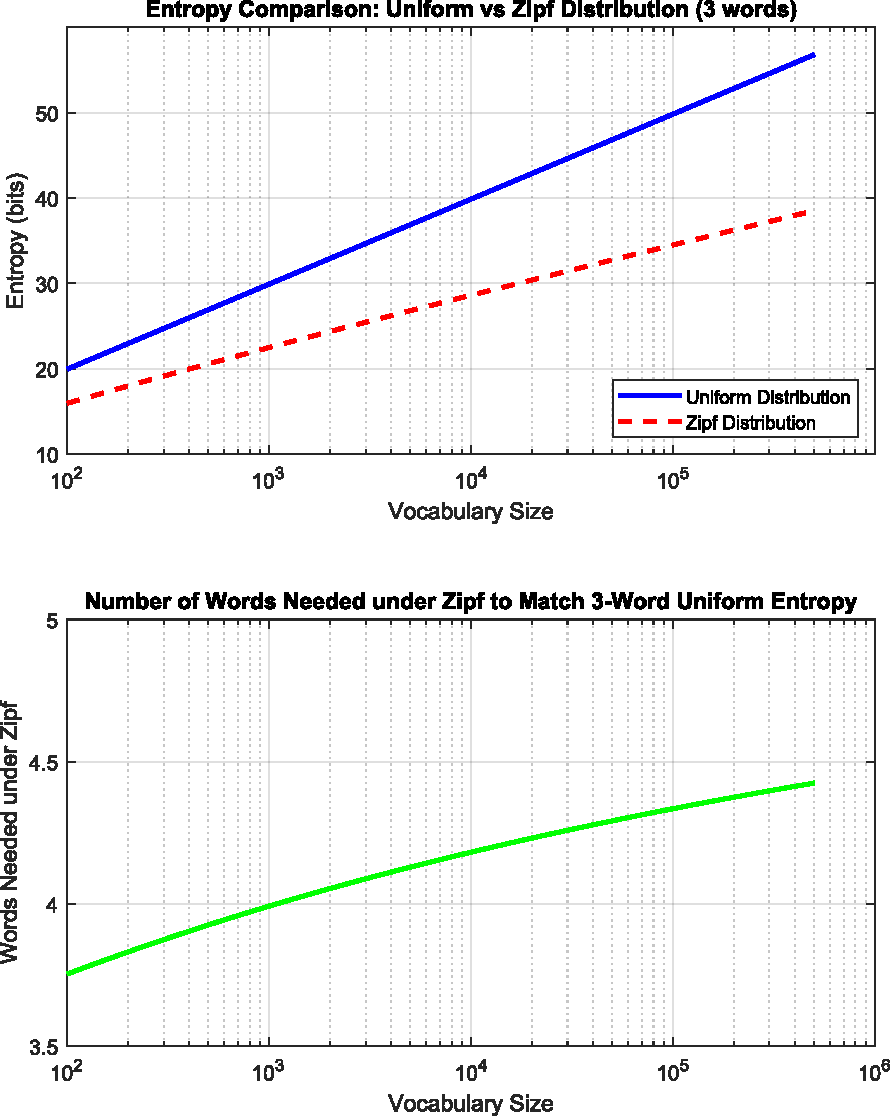
\includegraphics[scale=0.8]{figs/why_passwords/ncsc_threewords_diff.pdf}
        \caption{Chart showing the equivalent number of words required in practice to match the theoretical complexity of the National Cyber Security Centre's (NCSC) password composition policy. The NCSC recommends at least three random words, using our model we show that in practice a minium of 4 words is more secure. \srcOwnFig}
        \label{fig::chp4::zipfslaw-ncsc}
        \vspace*{-0.5cm}
    \end{figure}
   To align the password policy with enhanced entropy under Zipf's law, we need to determine the minimum number of words \( n \) required to achieve a desired entropy \( H_{\text{desired}} \). This can be formulated as:
   \[
n \geq \frac{H_{\text{desired}}}{H_{\text{word}}}
   \]
   Given that \( H_{\text{word}} \) is lower under Zipf's law compared to a uniform distribution (due to the presence of highly probable words), a larger \( n \) may be required to achieve the same entropy.
   
   Under a uniform distribution where each word has \( P(w) = \frac{1}{|\mathcal{W}|} \), the entropy per word is:
   $$H_{\text{word}}^{\text{uniform}} = \log |\mathcal{W}|$$
   Comparing with Zipf's law:
   \[
H_{\text{word}}^{\text{Zipf}} < H_{\text{word}}^{\text{uniform}}
   \]
   
   Zipf's law requires more words than a uniform distribution to achieve the same entropy level. As Figure~\ref{fig::chp4::zipfslaw-ncsc} demonstrates, when we increase the vocabulary size, the entropy difference between uniform and Zipf's distributions also increases. This comparison leads us to conclude that we need at least 4-5 words to match the entropy that NCSC's theoretical PCP describes. Moreover, this minimum word requirement grows as the vocabulary expands.

To maintain or exceed the entropy level recommended by NCSC using three random words under a Zipfian distribution, the policy should be adjusted to:
   \[
n_{\text{adjusted}} \geq \frac{3 \cdot \log |\mathcal{W}|}{H_{\text{word}}^{\text{Zipf}}}
   \]
   
   This ensures that the password composition maintains sufficient entropy despite the skewed word frequency distribution.
   
\subsubsection{Adjusted Password Structure Probability}

   If we adjust the structure to use \( n \) words to counteract the lowered entropy per word, the structure probability becomes:
   \begin{equation}
P(S_n) = \prod_{i=1}^{n} P(w_i) = \left( \frac{1}{\sum_{k=1}^{|\mathcal{W}|} 1 / k^s} \right)^n \prod_{i=1}^{n} \frac{1}{r_i^s}
   \end{equation}
   
   Ensuring that \( n \) is sufficiently large to maintain high entropy despite the non-uniform word distribution.



%\subsubsection{Optimizing Password Composition Policy}
%
%   The optimization objective can be revised to account for the Zipfian distribution of word selection:
%   \[
%\max_{n} H = n \cdot H_{\text{word}} \quad \text{subject to} \quad H \geq H_{\text{min}}
%   \]
%   
%   Where \( H_{\text{min}} \) is the minimum required entropy for password security.

%\subsubsection{Comparison with Uniform Distribution}
%
%   Under a uniform distribution where each word has \( P(w) = \frac{1}{|\mathcal{W}|} \), the entropy per word is:
%   \[
%H_{\text{word}}^{\text{uniform}} = \log |\mathcal{W}|
%   \]
%   
%
%\subsubsection{Final Policy Adjustment}
%
%   To maintain or exceed the entropy level recommended by NCSC using three random words under a Zipfian distribution, the policy should be adjusted to:
%   \[
%n_{\text{adjusted}} \geq \frac{3 \cdot \log |\mathcal{W}|}{H_{\text{word}}^{\text{Zipf}}}
%   \]
%   
%   This ensures that the password composition maintains sufficient entropy despite the skewed word frequency distribution.

% \subsection{UX Proposal}
% The NCSC's proposal is ambitious as users are likely to choose non-uniform words. This is a work in progress solution that combines UX flows with the NCSC PCP.
% 
% We provide the user with at least three input boxes (this is to ensure they use at least three words), and also ask them to remember a randomly generated digit.
% 
%\subsection{Dataset Complexity}

To maximize the complexity of the entire password dataset by considering the distribution of password structures, we can formulate an optimization problem that balances the diversity of structures with the entropy contributed by each structure. Below is a theoretical mathematical framework to address this scenario.

\subsubsection{Definitions and Notations}

\paragraph{Password Structure} Let \( \mathcal{S} = \{ S_1, S_2, \dots, S_m \} \) be the set of all possible password structures, where each structure \( S_j \) is a sequence of elements from the alphabet \( \Sigma \). For example, \( S_j = (w, w, d) \) represents a structure with two words followed by a digit.

\paragraph{Probability of a Structure} Let \( P(S_j) \) denote the probability of selecting structure \( S_j \) in the password dataset. Thus, the structure probabilities satisfy:
  \[
  \sum_{j=1}^{m} P(S_j) = 1
  \]

\paragraph{Elements within Structures} For a given structure \( S_j = (e_1, e_2, \dots, e_k) \), each element \( e_i \in \Sigma \) has an associated probability \( P(e_i \mid S_j) \).

\subsubsection{Password Probability Distribution}

The probability of a password \( p \) with structure \( S_j \) is given by:
\[
P(p) = P(S_j) \prod_{i=1}^{k} P(e_i \mid S_j)
\]
where \( p = (e_1, e_2, \dots, e_k) \).

\subsubsection{Entropy of the Password Dataset}

The entropy \( H \) of the entire password dataset, which measures its complexity, is defined as:
\[
H = - \sum_{j=1}^{m} P(S_j) \sum_{p \in S_j} P(p) \log P(p)
\]
Expanding \( P(p) \):
\begin{multline}
H = - \sum_{j=1}^{m} P(S_j) \sum_{p \in S_j} \left( P(S_j) \prod_{i=1}^{k} P(e_i \mid S_j) \right) \\ \log \left( P(S_j) \prod_{i=1}^{k} P(e_i \mid S_j) \right)
\end{multline}
Simplifying:
\[
H = - \sum_{j=1}^{m} P(S_j) \left[ \log P(S_j) + \sum_{i=1}^{k} \mathbb{E}_{e_i \mid S_j} [\log P(e_i \mid S_j)] \right]
\]
\[
H = - \sum_{j=1}^{m} P(S_j) \log P(S_j) - \sum_{j=1}^{m} P(S_j) \sum_{i=1}^{k} \mathbb{E}_{e_i \mid S_j} [\log P(e_i \mid S_j)]
\]
This can be expressed as:
\begin{equation}
H = H(\mathcal{S}) + \sum_{j=1}^{m} P(S_j) H(\mathcal{E} \mid S_j)
\end{equation}
where:

 \( H(\mathcal{S}) = - \sum_{j=1}^{m} P(S_j) \log P(S_j) \) is the entropy of the structure distribution.
 
\( H(\mathcal{E} \mid S_j) = - \sum_{i=1}^{k} \mathbb{E}_{e_i \mid S_j} [\log P(e_i \mid S_j)] \) is the conditional entropy of the elements given the structure \( S_j \).

\subsubsection{Optimization Objective}

To maximize the complexity \( H \) of the entire password dataset, we aim to maximize both the entropy of the structure distribution and the conditional entropy of elements within each structure. The optimization problem can be formulated as:
\begin{equation}
\max_{ \{ P(S_j), P(e_i \mid S_j) \} } H = H(\mathcal{S}) + \sum_{j=1}^{m} P(S_j) H(\mathcal{E} \mid S_j)
\end{equation}

**Subject to:**
1. **Probability Constraints:**
   \[
   \sum_{j=1}^{m} P(S_j) = 1
   \]
   \[
   \sum_{e_i \in S_j} P(e_i \mid S_j) = 1 \quad \forall j = 1, 2, \dots, m
   \]

2. **Structural Constraints:**
   - **Complexity Requirements:** Enforce minimum complexity for certain structures, e.g., ensuring that structures chosen have a minimal number of elements.
   - **Semantic Constraints:** Limit or regulate semantic relationships to avoid overly predictable patterns.

\subsubsection{Implications of Fixed vs. Random Structures}

\paragraph{Fixed Structure (e.g., \( S^* = (w, w, w) \))}

  If all users adopt a fixed structure \( S^* \), the structure entropy \( H(\mathcal{S}) \) becomes zero since \( P(S^*) = 1 \) and \( P(S_j) = 0 \) for \( j \neq * \). The overall entropy simplifies to:
  \[
  H = H(\mathcal{E} \mid S^*)
  \]
  This restricts complexity to the variability within the fixed structure, potentially limiting overall entropy.

\paragraph{Randomized Structures}

  Allowing multiple structures to be used with varying probabilities increases \( H(\mathcal{S}) \), thereby contributing to higher overall entropy. However, if structures vary randomly without enforcing complexity, many users might still choose less complex structures, resulting in lower \( H(\mathcal{E} \mid S_j) \) for those structures.

\subsubsection{Balancing Structure Distribution for Maximum Complexity}

To maximize \( H \), we need to optimally distribute \( P(S_j) \) across different structures, favouring structures that contribute higher conditional entropy \( H(\mathcal{E} \mid S_j) \). This can be formalized as:

\[
\max_{ \{ P(S_j) \} } H = - \sum_{j=1}^{m} P(S_j) \log P(S_j) + \sum_{j=1}^{m} P(S_j) H(\mathcal{E} \mid S_j)
\]

**Subject to:**
\[
\sum_{j=1}^{m} P(S_j) = 1
\]
\[
P(S_j) \geq 0 \quad \forall j
\]

This optimization encourages a diverse set of structures, each contributing positively to the overall entropy.

\subsubsection{Strategic Structure Allocation}

To ensure that the password dataset achieves high complexity, allocate higher probabilities to structures that inherently provide higher conditional entropy. For example:

- **High-Complexity Structures:** Structures with diverse elements (e.g., multiple words, mixed character types) can be assigned higher \( P(S_j) \).
  
- **Low-Complexity Structures:** Structures that are simple or have predictable patterns should have lower \( P(S_j) \).

Mathematically, this can be approached by defining an objective function that weighs structures based on their \( H(\mathcal{E} \mid S_j) \):

\[
P(S_j) \propto e^{\lambda H(\mathcal{E} \mid S_j)}
\]
where \( \lambda \) is a scaling parameter that controls the emphasis on entropy.

\subsubsection{Example with Zipf’s Law for Element Distribution}

Assuming elements within structures follow Zipf’s law, the conditional entropy \( H(\mathcal{E} \mid S_j) \) for a structure \( S_j \) can be computed as:

\[
H(\mathcal{E} \mid S_j) = - \sum_{e_i \in \Sigma_j} P(e_i \mid S_j) \log P(e_i \mid S_j)
\]
where \( \Sigma_j \) is the set of possible elements for structure \( S_j \).

Given Zipf’s law:
\[
P(e_i \mid S_j) = \frac{1 / r_i^s}{\sum_{k=1}^{|\Sigma_j|} 1 / k^s}
\]
the entropy becomes:
\[
H(\mathcal{E} \mid S_j) = \log \left( \sum_{k=1}^{|\Sigma_j|} \frac{1}{k^s} \right) + s \frac{\sum_{e_i \in \Sigma_j} \frac{\log r_i}{r_i^s}}{\sum_{k=1}^{|\Sigma_j|} \frac{1}{k^s}}
\]

\subsubsection{Implications for Password Policy Design}

\begin{itemize}
\item Avoiding Uniform Structure Assignment: Mandating a single structure (e.g., three words) can reduce overall entropy, making passwords more predictable if attackers exploit the fixed structure.
\item Encouraging Structure Diversity: Allowing a variety of structures with probabilities tuned to maximize overall entropy ensures that while some users may use simpler structures, others utilize more complex ones, increasing the average complexity of the dataset.
\item Ensuring Minimum Complexity: Introduce constraints to ensure that each structure contributes a minimum amount of entropy, preventing the selection of overly simplistic structures.
\end{itemize}

\subsubsection{Conclusion and Policy Recommendation}

To maximize the complexity of the entire password dataset:
\begin{enumerate}
\item Adopt a Diverse Structure Policy: Allow multiple password structures rather than enforcing a single structure like three words. This diversity increases \( H(\mathcal{S}) \) and, when combined with appropriate \( H(\mathcal{E} \mid S_j) \), enhances overall dataset complexity.

\item Optimize Structure Probabilities: Allocate higher probabilities to structures that offer higher conditional entropy, ensuring that more complex structures are prevalent.

\item Incorporate Entropy Constraints: Ensure that each allowed structure meets a minimum entropy threshold to prevent the prevalence of weak password structures.

\item Monitor and Adjust: Continuously analyze the password dataset to adjust structure probabilities and permitted structures in response to emerging patterns and threats.
\end{enumerate}
By strategically managing the distribution of password structures and their associated element complexities, the password policy can achieve maximal dataset complexity, enhancing security across the user base.

%\subsection{Memorability}

To design an effective password composition policy that balances \textbf{complexity} (entropy) and \textbf{memorability} (ease of understanding), we can formulate a multi-objective optimization framework. This framework integrates measures of both complexity and memorability to derive an optimal policy that maximizes security while ensuring usability for users.

### 1. **Definitions and Notations**

- **Password Structure Set**: Let \( \mathcal{S} = \{ S_1, S_2, \dots, S_m \} \) denote the set of all possible password structures, where each structure \( S_j \) is a sequence of elements from the alphabet \( \Sigma \). For example, \( S_j = (w, w, d) \) represents a structure with two words followed by a digit.

- **Probability of a Structure**: Let \( P(S_j) \) denote the probability of selecting structure \( S_j \) in the password dataset. The structure probabilities satisfy:
  \[
  \sum_{j=1}^{m} P(S_j) = 1
  \]

- **Elements within Structures**: For a given structure \( S_j = (e_1, e_2, \dots, e_k) \), each element \( e_i \in \Sigma \) has an associated probability \( P(e_i \mid S_j) \).

- **Entropy (Complexity)**: The entropy \( H \) of the password dataset measures its complexity and is defined as:
  \[
  H = H(\mathcal{S}) + \sum_{j=1}^{m} P(S_j) H(\mathcal{E} \mid S_j)
  \]
  where:
  \[
  H(\mathcal{S}) = - \sum_{j=1}^{m} P(S_j) \log P(S_j)
  \]
  and
  \[
  H(\mathcal{E} \mid S_j) = - \sum_{e_i \in \Sigma_j} P(e_i \mid S_j) \log P(e_i \mid S_j)
  \]

- **Memorability Measure**: Let \( M \) denote the memorability of the password dataset. We define \( M \) as a function that quantifies the ease with which users can remember their passwords. For mathematical modeling, \( M \) can be represented as:
  \[
  M = \sum_{j=1}^{m} P(S_j) M(S_j)
  \]
  where \( M(S_j) \) is the memorability score of structure \( S_j \). Higher values of \( M \) indicate greater memorability.

### 2. **Multi-Objective Optimization Framework**

To balance complexity and memorability, we define an objective function that incorporates both \( H \) and \( M \). This can be achieved through a weighted sum approach or by setting constraints.

#### a. **Weighted Sum Approach**

Define a weight parameter \( \lambda \in [0, 1] \) that balances the importance between complexity and memorability. The objective function \( \mathcal{O} \) to be maximized is:
\[
\mathcal{O} = H + \lambda M
\]
Substituting the definitions of \( H \) and \( M \):
\[
\mathcal{O} = \left[ H(\mathcal{S}) + \sum_{j=1}^{m} P(S_j) H(\mathcal{E} \mid S_j) \right] + \lambda \left[ \sum_{j=1}^{m} P(S_j) M(S_j) \right]
\]
The optimization problem becomes:
\[
\max_{\{ P(S_j), P(e_i \mid S_j) \}} \mathcal{O} = H + \lambda M
\]
**Subject to:**
\[
\sum_{j=1}^{m} P(S_j) = 1
\]
\[
\sum_{e_i \in S_j} P(e_i \mid S_j) = 1 \quad \forall j = 1, 2, \dots, m
\]
\[
P(S_j) \geq 0 \quad \forall j
\]
\[
P(e_i \mid S_j) \geq 0 \quad \forall e_i, S_j
\]

#### b. **Constrained Optimization Approach**

Alternatively, we can maximize complexity \( H \) while ensuring that memorability \( M \) meets a minimum threshold \( M_{\text{min}} \):
\[
\max_{\{ P(S_j), P(e_i \mid S_j) \}} H
\]
**Subject to:**
\[
M \geq M_{\text{min}}
\]
\[
\sum_{j=1}^{m} P(S_j) = 1
\]
\[
\sum_{e_i \in S_j} P(e_i \mid S_j) = 1 \quad \forall j
\]
\[
P(S_j) \geq 0 \quad \forall j
\]
\[
P(e_i \mid S_j) \geq 0 \quad \forall e_i, S_j
\]

### 3. **Modeling the Memorability Function \( M(S_j) \)**

The memorability of a structure \( S_j \) can be modeled based on several factors, such as:

- **Simplicity of Structure**: Structures with fewer and more familiar elements (e.g., common words) are generally more memorable.
- **Semantic Relationships**: Structures where elements have meaningful or coherent relationships may enhance memorability.
- **Pattern Regularity**: Structures with regular patterns or repetitions may be easier to remember.

Mathematically, \( M(S_j) \) can be expressed as:
\[
M(S_j) = \alpha \cdot f_{\text{simplicity}}(S_j) + \beta \cdot f_{\text{semantic}}(S_j) + \gamma \cdot f_{\text{pattern}}(S_j)
\]
where \( \alpha, \beta, \gamma \) are weighting coefficients that balance the contribution of each factor, and:
\[
f_{\text{simplicity}}(S_j) = \text{Function quantifying simplicity}
\]
\[
f_{\text{semantic}}(S_j) = \text{Function quantifying semantic coherence}
\]
\[
f_{\text{pattern}}(S_j) = \text{Function quantifying pattern regularity}
\]

### 4. **Incorporating Constraints for Policy Design**

To ensure that the password composition policy is practical and enforceable, we may incorporate additional constraints such as:

- **Minimum and Maximum Structure Length**:
  \[
  k_{\text{min}} \leq |S_j| \leq k_{\text{max}} \quad \forall S_j \in \mathcal{S}
  \]
  where \( |S_j| \) denotes the number of elements in structure \( S_j \).

- **Prohibited Patterns or Elements**:
  \[
  P(e_i \mid S_j) = 0 \quad \text{for prohibited } e_i \text{ in structure } S_j
  \]

- **Minimum Entropy Requirements**:
  \[
  H \geq H_{\text{min}}
  \]

### 5. **Strategy for Designing the Password Composition Policy**

Based on the above framework, the strategy to design the password composition policy involves the following steps:

#### a. **Define the Structure Set \( \mathcal{S} \)**
Determine the allowable password structures based on desired elements (e.g., words, numbers, symbols) and their sequence.

#### b. **Model Complexity and Memorability**
- **Complexity**: Calculate the entropy \( H \) for each structure and the overall dataset.
- **Memorability**: Define and compute the memorability function \( M(S_j) \) for each structure.

#### c. **Formulate the Optimization Problem**
Decide on the objective (e.g., maximize \( H + \lambda M \) or maximize \( H \) subject to \( M \geq M_{\text{min}} \)) and set up the corresponding optimization problem.

#### d. **Solve the Optimization Problem**
Determine the optimal structure probabilities \( P(S_j) \) and element probabilities \( P(e_i \mid S_j) \) that achieve the desired balance between complexity and memorability.

#### e. **Implement Policy Constraints**
Incorporate practical constraints to ensure the policy is user-friendly and enforceable.

#### f. **Iterative Refinement**
Continuously monitor password usage and feedback to adjust the policy parameters \( \lambda \), \( \alpha \), \( \beta \), \( \gamma \), and the structure set \( \mathcal{S} \) to optimize both security and usability.

### 6. **Illustrative Example**

Consider a simplified scenario with two possible structures:
- \( S_1 = (w, w, w) \) (three words)
- \( S_2 = (w, d, s) \) (word, digit, symbol)

Assume the following for memorability:
\[
M(S_1) = 0.8 \quad \text{and} \quad M(S_2) = 0.6
\]

And entropy calculations:
\[
H(\mathcal{S}) = - P(S_1) \log P(S_1) - P(S_2) \log P(S_2)
\]
\[
H(\mathcal{E} \mid S_1) = H_{\text{words}} \quad \text{and} \quad H(\mathcal{E} \mid S_2) = H_{\text{word}} + H_{\text{digit}} + H_{\text{symbol}}
\]

Using the weighted sum approach with \( \lambda = 0.5 \):
\[
\mathcal{O} = H(\mathcal{S}) + P(S_1) H_{\text{words}} + P(S_2) (H_{\text{word}} + H_{\text{digit}} + H_{\text{symbol}}) + 0.5 [P(S_1) \cdot 0.8 + P(S_2) \cdot 0.6]
\]

Solving the optimization problem would yield the optimal probabilities \( P(S_1) \) and \( P(S_2) \) that maximize \( \mathcal{O} \), thereby balancing complexity and memorability.

### 7. **Conclusion and Policy Recommendation**

To design a robust password composition policy for your website that maximizes security while ensuring ease of use:

1. **Integrate Complexity and Memorability**: Utilize a multi-objective optimization framework that considers both entropy (complexity) and a defined memorability measure.

2. **Diversify Structure Probabilities**: Allow a variety of password structures with probabilities optimized to balance entropy and memorability. Avoid enforcing a single structure (e.g., three words) to prevent predictability and potential entropy reduction.

3. **Optimize Structure Selection**: Allocate higher probabilities to structures that offer higher entropy and sufficient memorability, ensuring that users are encouraged to adopt strong yet memorable password formats.

4. **Set Practical Constraints**: Incorporate constraints to maintain usability, such as limiting structure complexity to manageable levels and ensuring that all allowed structures meet minimum security requirements.

5. **Continuous Evaluation and Adjustment**: Regularly assess the effectiveness of the password policy by analyzing password entropy and user feedback on memorability, adjusting the policy parameters as necessary to maintain an optimal balance.

By adopting this strategic, mathematically grounded approach, your website can implement a password composition policy that enhances security through high-entropy passwords while maintaining user-friendly memorability.


%\subsection{Random Word}
%To analyze the impact of incorporating an additional uniformly random word into the password composition policy (PCP), we will extend the existing framework to account for this modification. Specifically, we consider a PCP that requires:
%
%1. **Minimum of Three Words**: Users must select at least three words.
%2. **Minimum Length of 10 Characters**: The total length of the password must be at least 10 characters.
%3. **Addition of a System-Generated Random Word**: A uniformly random word is appended to the user's selected words.
%
%### 1. **Revised Password Structure**
%
%Let \( S \) denote the original password structure comprising three words. The revised structure \( S' \) includes the additional system-generated random word:
%
%\[
%S' = (w_1, w_2, w_3, w_r)
%\]
%
%where:
%- \( w_1, w_2, w_3 \) are user-selected words.
%- \( w_r \) is the system-generated uniformly random word.
%
%### 2. **Probability of the Revised Structure \( S' \)**
%
%Assuming that the user selects words independently and the system-generated word is chosen uniformly from the vocabulary \( \mathcal{W} \), the probability of a specific password \( p' \) with structure \( S' \) is:
%
%\[
%P(p') = P(w_1, w_2, w_3, w_r) = P(w_1) \cdot P(w_2) \cdot P(w_3) \cdot P(w_r)
%\]
%
%Given that \( w_r \) is uniformly random:
%
%\[
%P(w_r) = \frac{1}{|\mathcal{W}|}
%\]
%
%Thus,
%
%\[
%P(p') = P(w_1) \cdot P(w_2) \cdot P(w_3) \cdot \frac{1}{|\mathcal{W}|}
%\]
%
%### 3. **Entropy of the Revised Password Distribution**
%
%The entropy \( H' \) of the revised password distribution \( P' \) incorporating the system-generated random word is defined as:
%
%\[
%H' = -\sum_{p' \in \mathcal{P}'} P(p') \log P(p')
%\]
%
%Substituting \( P(p') \):
%
%\[
%H' = -\sum_{w_1, w_2, w_3, w_r \in \mathcal{W}} \left( P(w_1) \cdot P(w_2) \cdot P(w_3) \cdot \frac{1}{|\mathcal{W}|} \right) \log \left( P(w_1) \cdot P(w_2) \cdot P(w_3) \cdot \frac{1}{|\mathcal{W}|} \right)
%\]
%
%Expanding the logarithm:
%
%\[
%H' = -\sum_{w_1, w_2, w_3, w_r \in \mathcal{W}} \left( P(w_1) \cdot P(w_2) \cdot P(w_3) \cdot \frac{1}{|\mathcal{W}|} \right) \left( \log P(w_1) + \log P(w_2) + \log P(w_3) + \log \left( \frac{1}{|\mathcal{W}|} \right) \right)
%\]
%
%This can be separated into:
%
%\[
%H' = H(S) + H(w_r)
%\]
%
%where:
%- \( H(S) \) is the entropy of the original structure \( S \) (three user-selected words).
%- \( H(w_r) \) is the entropy contributed by the uniformly random word.
%
%**Entropy of the Original Structure \( S \):**
%
%\[
%H(S) = -\sum_{w_1, w_2, w_3 \in \mathcal{W}} P(w_1) \cdot P(w_2) \cdot P(w_3) \log \left( P(w_1) \cdot P(w_2) \cdot P(w_3) \right)
%\]
%
%Expanding:
%
%\[
%H(S) = -\sum_{w_1, w_2, w_3 \in \mathcal{W}} P(w_1) \cdot P(w_2) \cdot P(w_3) \left( \log P(w_1) + \log P(w_2) + \log P(w_3) \right)
%\]
%
%\[
%H(S) = 3 \cdot H_{\text{word}}
%\]
%
%where:
%
%\[
%H_{\text{word}} = -\sum_{w \in \mathcal{W}} P(w) \log P(w)
%\]
%
%**Entropy of the Uniformly Random Word \( w_r \):**
%
%\[
%H(w_r) = -\sum_{w_r \in \mathcal{W}} P(w_r) \log P(w_r) = \log |\mathcal{W}|
%\]
%
%since \( P(w_r) = \frac{1}{|\mathcal{W}|} \).
%
%**Total Entropy \( H' \):**
%
%\[
%H' = 3 \cdot H_{\text{word}} + \log |\mathcal{W}|
%\]
%
%### 4. **Impact on Password Complexity**
%
%The addition of a uniformly random word \( w_r \) increases the overall entropy of the password distribution by \( \log |\mathcal{W}| \), thereby enhancing the complexity of each password. The total entropy \( H' \) is the sum of the entropy from the user-selected words and the entropy from the system-generated word.
%
%### 5. **Overall Password Distribution**
%
%The revised password distribution \( P' \) is a convolution of the user-selected word distribution and the uniform distribution of the system-generated word. Formally, the joint probability distribution can be expressed as:
%
%\[
%P'(w_1, w_2, w_3, w_r) = P(w_1, w_2, w_3) \cdot P(w_r)
%\]
%
%Given independence:
%
%\[
%P'(w_1, w_2, w_3, w_r) = P(w_1) \cdot P(w_2) \cdot P(w_3) \cdot \frac{1}{|\mathcal{W}|}
%\]
%
%### 6. **Entropy Comparison**
%
%**Original Entropy \( H \) (Three User-Selected Words):**
%
%\[
%H = 3 \cdot H_{\text{word}}
%\]
%
%**Revised Entropy \( H' \) (Three User-Selected Words + One Uniform Word):**
%
%\[
%H' = 3 \cdot H_{\text{word}} + \log |\mathcal{W}|
%\]
%
%**Difference in Entropy:**
%
%\[
%\Delta H = H' - H = \log |\mathcal{W}|
%\]
%
%This indicates that the entropy increases by \( \log |\mathcal{W}| \) when a uniformly random word is appended to the password.
%
%### 7. **Effect on Password Distribution**
%
%The incorporation of a uniformly random word \( w_r \) affects the overall password distribution in the following ways:
%
%1. **Increased Uniformity**: The uniform distribution of \( w_r \) introduces a component of uniform randomness to the password, mitigating the skewness introduced by the user-selected words (which may follow Zipf's law or another non-uniform distribution).
%
%2. **Diversification of Structures**: By appending a uniformly random word, the effective structure becomes slightly more complex, as it introduces an element that is independent of the user-selected words.
%
%3. **Overall Distribution Shift**: The joint distribution becomes a product of the original non-uniform distribution (from user-selected words) and a uniform distribution, leading to a more balanced overall distribution.
%
%Formally, if the original password distribution \( P(S) \) is skewed, the revised distribution \( P'(S') \) incorporates an additional uniform factor, reducing the overall skewness:
%
%\[
%P'(S') = P(S) \cdot P(w_r) = P(w_1, w_2, w_3) \cdot \frac{1}{|\mathcal{W}|}
%\]
%
%### 8. **Implications for Password Composition Policy**
%
%1. **Enhanced Security**: The increase in entropy \( \Delta H = \log |\mathcal{W}| \) directly translates to higher password complexity, making passwords more resistant to brute-force and dictionary attacks.
%
%2. **Distribution Uniformity**: The addition of a uniformly random word helps in flattening the probability distribution of passwords, ensuring that no single password structure overwhelmingly dominates, thus reducing predictability.
%
%3. **User Compliance and Usability**: While enhancing security, it's essential to consider the impact on user experience. Appending a system-generated random word should be implemented in a manner that maintains or even improves memorability, possibly by selecting easily memorable words or using mechanisms like passphrases.
%
%4. **Minimum Length Enforcement**: The constraint of a minimum length of 10 characters ensures that even with shorter words, the appended random word contributes significantly to reaching the desired complexity.
%
%### 9. **Summary of Mathematical Framework**
%
%To encapsulate the above analysis, the revised password composition policy can be modeled as follows:
%
%1. **Password Structure \( S' \)**:
%
%\[
%S' = (w_1, w_2, w_3, w_r)
%\]
%
%2. **Probability of Password \( p' \)**:
%
%\[
%P(p') = P(w_1) \cdot P(w_2) \cdot P(w_3) \cdot \frac{1}{|\mathcal{W}|}
%\]
%
%3. **Entropy \( H' \)**:
%
%\[
%H' = 3 \cdot H_{\text{word}} + \log |\mathcal{W}|
%\]
%
%4. **Overall Distribution \( P' \)**:
%
%\[
%P'(w_1, w_2, w_3, w_r) = P(w_1) \cdot P(w_2) \cdot P(w_3) \cdot \frac{1}{|\mathcal{W}|}
%\]
%
%### 10. **Conclusion**
%
%By enforcing a minimum of three user-selected words and appending a uniformly random word, the password composition policy achieves a significant increase in entropy, thereby enhancing the overall complexity and security of passwords. Additionally, the introduction of a uniformly random word contributes to a more uniform password distribution, mitigating the risks associated with non-uniform word selection patterns such as those described by Zipf's law.
%
%This mathematical framework provides a solid foundation for evaluating and optimizing the password composition policy to strike an optimal balance between security (complexity) and usability (memorability).

%\subsection{Evaluation}
%\label{sec::chp4::pcp-evaluation}
%
%Passwords are structured using elements, such as $w^2d^3$ $\rightarrow$ \password{thepassword123}, this structure is referred to as $S$. We associate a probability of a sequence of structure $P(S)$. We also associate a probability of instances of elements holding semantic relationships (e.g. two common words).
%
%For a password p, we define its structure S as a sequence of elements from our alphabet:
%\begin{equation}
%S(p) = (e_1, ..., e_n), \text{ where } e_i \in \Sigma = {w, n, d, s, ...}
%\end{equation}
%Where w represents words, n names, d digits, and s special characters. The probability of observing a particular structure can be modeled using a first-order Markov chain:
%\begin{equation}
%P(S) = P(e_1)\prod_{i=2}^n P(e_i|e_{i-1})
%\end{equation}
%For semantic relationships between elements (particularly words and names), we introduce a semantic transition kernel K. For elements x, y ∈ V where V is our vocabulary:
%\begin{equation}
%K(x, y, t): \mathcal{V} \times \mathcal{V} \times \mathbb{R}^+ \rightarrow [0,1]
%\end{equation}
%This kernel satisfies the Chapman-Kolmogorov equation:
%\begin{equation}
%K(x, y, t+s) = \int_{\mathcal{V}} K(x, z, t)K(z, y, s),dz
%\end{equation}
%For practical computation, we can discretize this for our finite vocabulary:
%\begin{equation}
%K(x, y, t+s) = \sum_{z \in \mathcal{V}} K(x, z, t)K(z, y, s)
%\end{equation}
%The entropy of the password system can be decomposed into structural and semantic components:
%\begin{equation}
%H_{\text{total}} = H_{\text{struct}} + H_{\text{sem}}
%\end{equation}
%Where structural entropy is:
%\begin{equation}
%H_{\text{struct}} = -\sum_{S \in \mathcal{S}} P(S)\log_2 P(S)
%\end{equation}
%And semantic entropy, incorporating our transition kernel:
%\begin{equation}
%H_{\text{sem}} = -\sum_{x \in \mathcal{V}} \sum_{y \in \mathcal{V}} P(x)K(x, y, t)\log_2 K(x, y, t)
%\end{equation}
%To account for temporal evolution of password patterns, we introduce a time-dependent master equation:
%\begin{equation}
%\frac{\partial P(x,t)}{\partial t} = \int_{\mathcal{V}} [W(x|y)P(y,t) - W(y|x)P(x,t)],dy
%\end{equation}
%Where W(x|y) represents the transition rate from state y to x, and P(x,t) is the probability distribution over passwords at time t.
%The system's total guessing entropy can then be bounded by:
%\begin{equation}
%G \geq 2^{H_{\text{total}}-1}
%\end{equation}
%This provides a lower bound on the expected number of guesses required to crack a password in the system.
%
%\subsection{Memorability}
%\begin{equation}
%M(p, t) = \alpha M_{\text{struct}}(p) + (1-\alpha)M_{\text{sem}}(p)e^{-\lambda t}
%\end{equation}
%Where $\alpha \in$ [0,1] balances structural versus semantic memorability. The structural memorability can be modeled as:
%\begin{equation}
%M_{\text{struct}}(p) = \prod_{i=1}^n \phi(e_i) \psi(|e_i|)
%\end{equation}
%Here, $\phi(e_i)$ represents element-specific cognitive load and ψ(|e\_i|) captures length penalties. For semantic memorability:
%\begin{equation}
%M_{\text{sem}}(p) = \sum_{i=1}^{n-1} \gamma(e_i, e_{i+1})
%\end{equation}
%Where $\gamma$ measures semantic relatedness between adjacent elements. We can now define an optimality criterion that balances security and memorability:
%\begin{equation}
%Q(p) = \beta H_{\text{total}}(p) + (1-\beta)M(p,t)
%\end{equation}
%The decay parameter $\lambda$ follows a modified Ebbinghaus forgetting curve:
%\begin{equation}
%\lambda(r) = \lambda_0 e^{-\mu r}
%\end{equation}
%Where r represents rehearsal frequency and μ is a learning rate parameter. This gives us a complete framework for password strength that accounts for both security and cognitive constraints. The optimal password p* maximizes Q:
%\begin{equation}
%p^* = \argmax_{p \in \mathcal{P}} Q(p)
%\end{equation}
%Subject to minimal security constraints:
%\begin{equation}
%H_{\text{total}}(p) \geq H_{\text{min}}
%\end{equation}
%This formulation provides a principled way to generate passwords that are both secure and memorable, with tunable parameters α and β to adjust the security-memorability trade-off according to specific use cases


%\noteBox{Remark}{%
%We are considering human-memorable and generated passwords. In ideal scenarios, machine-generated passwords stored in password managers for example would offer greater security and scalability. So, this is not a comparison to a scenario where password managers are available to the user. We are considering this scenario because password managers are not widely adopted by a given population.
%}

%We can compare PCPs using two factors: usability and the strength given some PCP. Usability can be measured in the number of conditions and their difficulty. Strength given some PCP is a difficult and debated topic in the literature, however, here we use brute-force, dictionary attack, and the \zxcvbn PSM to measure strength.
%
%The usefulness of our data here is as follows. Instead of forcing the user to compose passwords with some rules without any knowledge of what the password structures could be like, and their expected strength. We can look at real passwords and discover the most secure structures. Then for each we can determine the conditions that would create such a secure password structure. Looking at it from this perspective, we find that the NCSC's \cite{ncsc2024} password recommendation of \textit{at least three random words} to be the most practical PCP.

% In this section, we will demonstrate why the NCSC's \cite{ncsc2024} password recommendation of \textit{at least three random words} stands as the most practical advice to date. Analysing passwords inevitably leads to considerations on how to forge secure passwords. The security level of a password, gauged through various strength or complexity metrics, is essentially governed by specific \textit{policies}. The discourse around password policy and complexity is extensive, with some asserting that passwords which are both human-chosen and memorable cannot be secure \cite{Weir_Aggarwal_Medeiros_Glodek_2009}. Here, we will examine these assertions using our labelled dataset as evidence.


% \begin{table}[h]
% \centering
% \caption{Password Policy Recommendations in Mathematical Notations}
% \begin{tabular}{|c|c|c|}
% \hline
% \textbf{Reference} & \textbf{Country} & \textbf{Guidelines and Recommendations} \\ \hline
% NIST (1985) & USA & \( L \geq 4, D = 1 \) \\ \hline
% NIST (2004) & USA & Level 2: \( L \geq 8 \), \( S = 1 \) \\ \hline
% BSI (2005) & DE & \( L \geq 8, D = 1, S = 1 \) \\ \hline
% US-CERT (2009) & USA & \( L \geq 8, U = 1, l = 1, D = 1, S = 1 \) \\ \hline
% DISA (2014) & USA & \( L \geq 15, U = 1, l = 1, D = 1, S = 1 \) \\ \hline
% NIST (2017) & USA & \( L \geq 8, C \geq 3 \) \\ \hline
% NCSC (2018) & UK & \( L \geq 8, C \geq 2 \) \\ \hline
% BSI (2019) & DE & \( L \geq 8, C \geq 2 \) \\ \hline
% BSI (2020) & DE & \( L \geq 8, C \geq 2 \) \\ \hline
% OWASP (2022) & - & \( L \geq 8, L \leq 64, S = 1 \) \\ \hline
% \end{tabular}
% \end{table}

%\subsection{Attack Model}
%\label{section:complexity:attack-model}

% We assume an offline attack scenario where the attacker has access to the hash value of the target's password--they are, therefore, not rate limited. The methods of attack deployed by the attacker, or the tools they use is inspired by what happens in practice. An example of such practice can be taken from the post-challenge report of Team Hashcat: Every year, KoreLogic \cite{noauthor_korelogic_nodate} hosts a password cracking challenge at the DEF CON conference \cite{tangent_defconorg_nodate}. Team Hashcat (the developers of the \hashcat password guessing software), have been the winners for the last 3  years. Their 2023 lineup consisted of 20 hackers, 47 FPGA boards, 78 GPUs and cloud infrastructure. Their post-challenge report \cite{noauthor_hashcatteam-hashcat_2023} is a good illustration of an attack strategy, especially given that the 2023's challenge was emulating a real world scenario. None of the prominent machine learning techniques were used except \pcfg in order to crack passphrases, which was trained on the existing cracked passphrases. Much of the manual work revolved around deciphering the underlying patterns in order to reduce the search space.

%Firstly, users tend to select words from a non-uniform distribution as shown in \S\ref{fig:word_freq_loglog}, significantly narrowing the search space and making passwords more predictable. This observation underscores the vulnerability of common password choices to guessing attacks. Secondly, the inherent structure of passwords—particularly those most commonly used—reveals considerable information, facilitating attacks like Probabilistic Context-Free Grammar (\pcfg). As detailed in Table \ref{table:structures}, the predominant password structures are $w$ (word) and $n$ (name), both of which are highly susceptible to dictionary attacks. Furthermore, the efficacy of these attacks varies with the hash function used. To illustrate, the table includes the time required to execute dictionary or hybrid attacks using consumer-level hardware across different hash functions, highlighting the practical implications of these security insights. We also compare this to a newer dataset--\lizardsquad (2015) as shown in Table \ref{table:ls-structures}.
%
%At the tail end of Table \ref{table:structures} and \ref{table:ls-structures} we see structures, such as $wwww$ (or $w^4$) that are resilient even if they were hashed using MD5. So, passwords comprising multiple words exhibit better security, withstanding hybrid attacks for extended duration, using the same hardware. However, their strength is compromised if the selected words have a high probabilistic correlation. In cases like the pattern \texttt{"mira que eres canalla”}, predictability increases significantly, as the words in the phrase have a relationship. But, most importantly the phrase is a popular song name in Spanish, which makes it even more predictable as a phrase.
% 
%
%To counteract this predictability, an effective strategy involves selecting words with minimal semantic or probabilistic linkage. Such a choice ensures that using an online corpus for predictive modelling yields low efficiency in guessing the subsequent word.
%
%Password policies can be classified as continuous, involving algorithms or probabilistic methods, which do not allow for concise user instructions on recommended password structures or word choices. Alternatively, password policies can be discrete, exemplified by the guidelines from NCSC \cite{ncsc2024} and NIST \cite{nist2024}, which are clearly defined. Our analysis, based on the \hmail dataset, supports the effectiveness of the NCSC \cite{ncsc2024} policy. Furthermore, our examination with \zxcvbn, as illustrated in Figure \ref{fig:heatmap_structure} and Table \ref{table:bin4}, indicates that the most secure structures involve multiple words, regardless of the probabilistic relationships between the words in this dataset. However, as we demonstrated using Eq. \ref{eq:pwi=0}, we should aim for no semantic relationship between the words.

% The analysis of password strength uses the entropy formula $E=log_2(R^L)$, with $R$ representing the possible characters and $L$ the password length. It shows that passwords, regardless of their complexity as measured by entropy, are still vulnerable to hybrid attacks (a mix of dictionary and brute-force tactics) on standard hardware. The study, considering a dictionary of 500,000 terms, suggests many passwords can be compromised by these attacks, highlighting that high entropy does not guarantee strong password security.

%In a Markov process for word sequences in passwords, the probability of a word sequence $W = \{w_1, w_2, w_3, w_4\}$ (where each $w_i$ represents a word) is given by the product of conditional probabilities:
%\begin{equation}
% P(W) = P(w_1) P(w_2 | w_1) P(w_3 | w_2) P(w_4 | w_3)
%\end{equation}
%For a strong password comprising multiple words, we aim for the condition that each word is independent of its preceding word. In such a case, the conditional probabilities should be equal to the individual probabilities of each word, i.e., $P(w_i | w_{i-1}) = P(w_i)$. Therefore, for a password of 4 words where each word is chosen independently we get Eq. \ref{eq:independent_stochastic_process}.
%\begin{equation}\label{eq:independent_stochastic_process}
%P(W) = P(w_1) P(w_2) P(w_3) P(w_4)
%\end{equation}
%In an ideal scenario where words are chosen with no semantic or probabilistic relationship to one another, the Markov probability chain should approach a condition where:
%\begin{equation}\label{eq:pwi=0}
%P(w_i | w_{i-1}) \approx 0\end{equation}
%Hence, for a 4-word password with maximally uncorrelated words, the overall probability of predicting the entire phrase should approach zero.

    \begin{figure}[t]
        \centering
        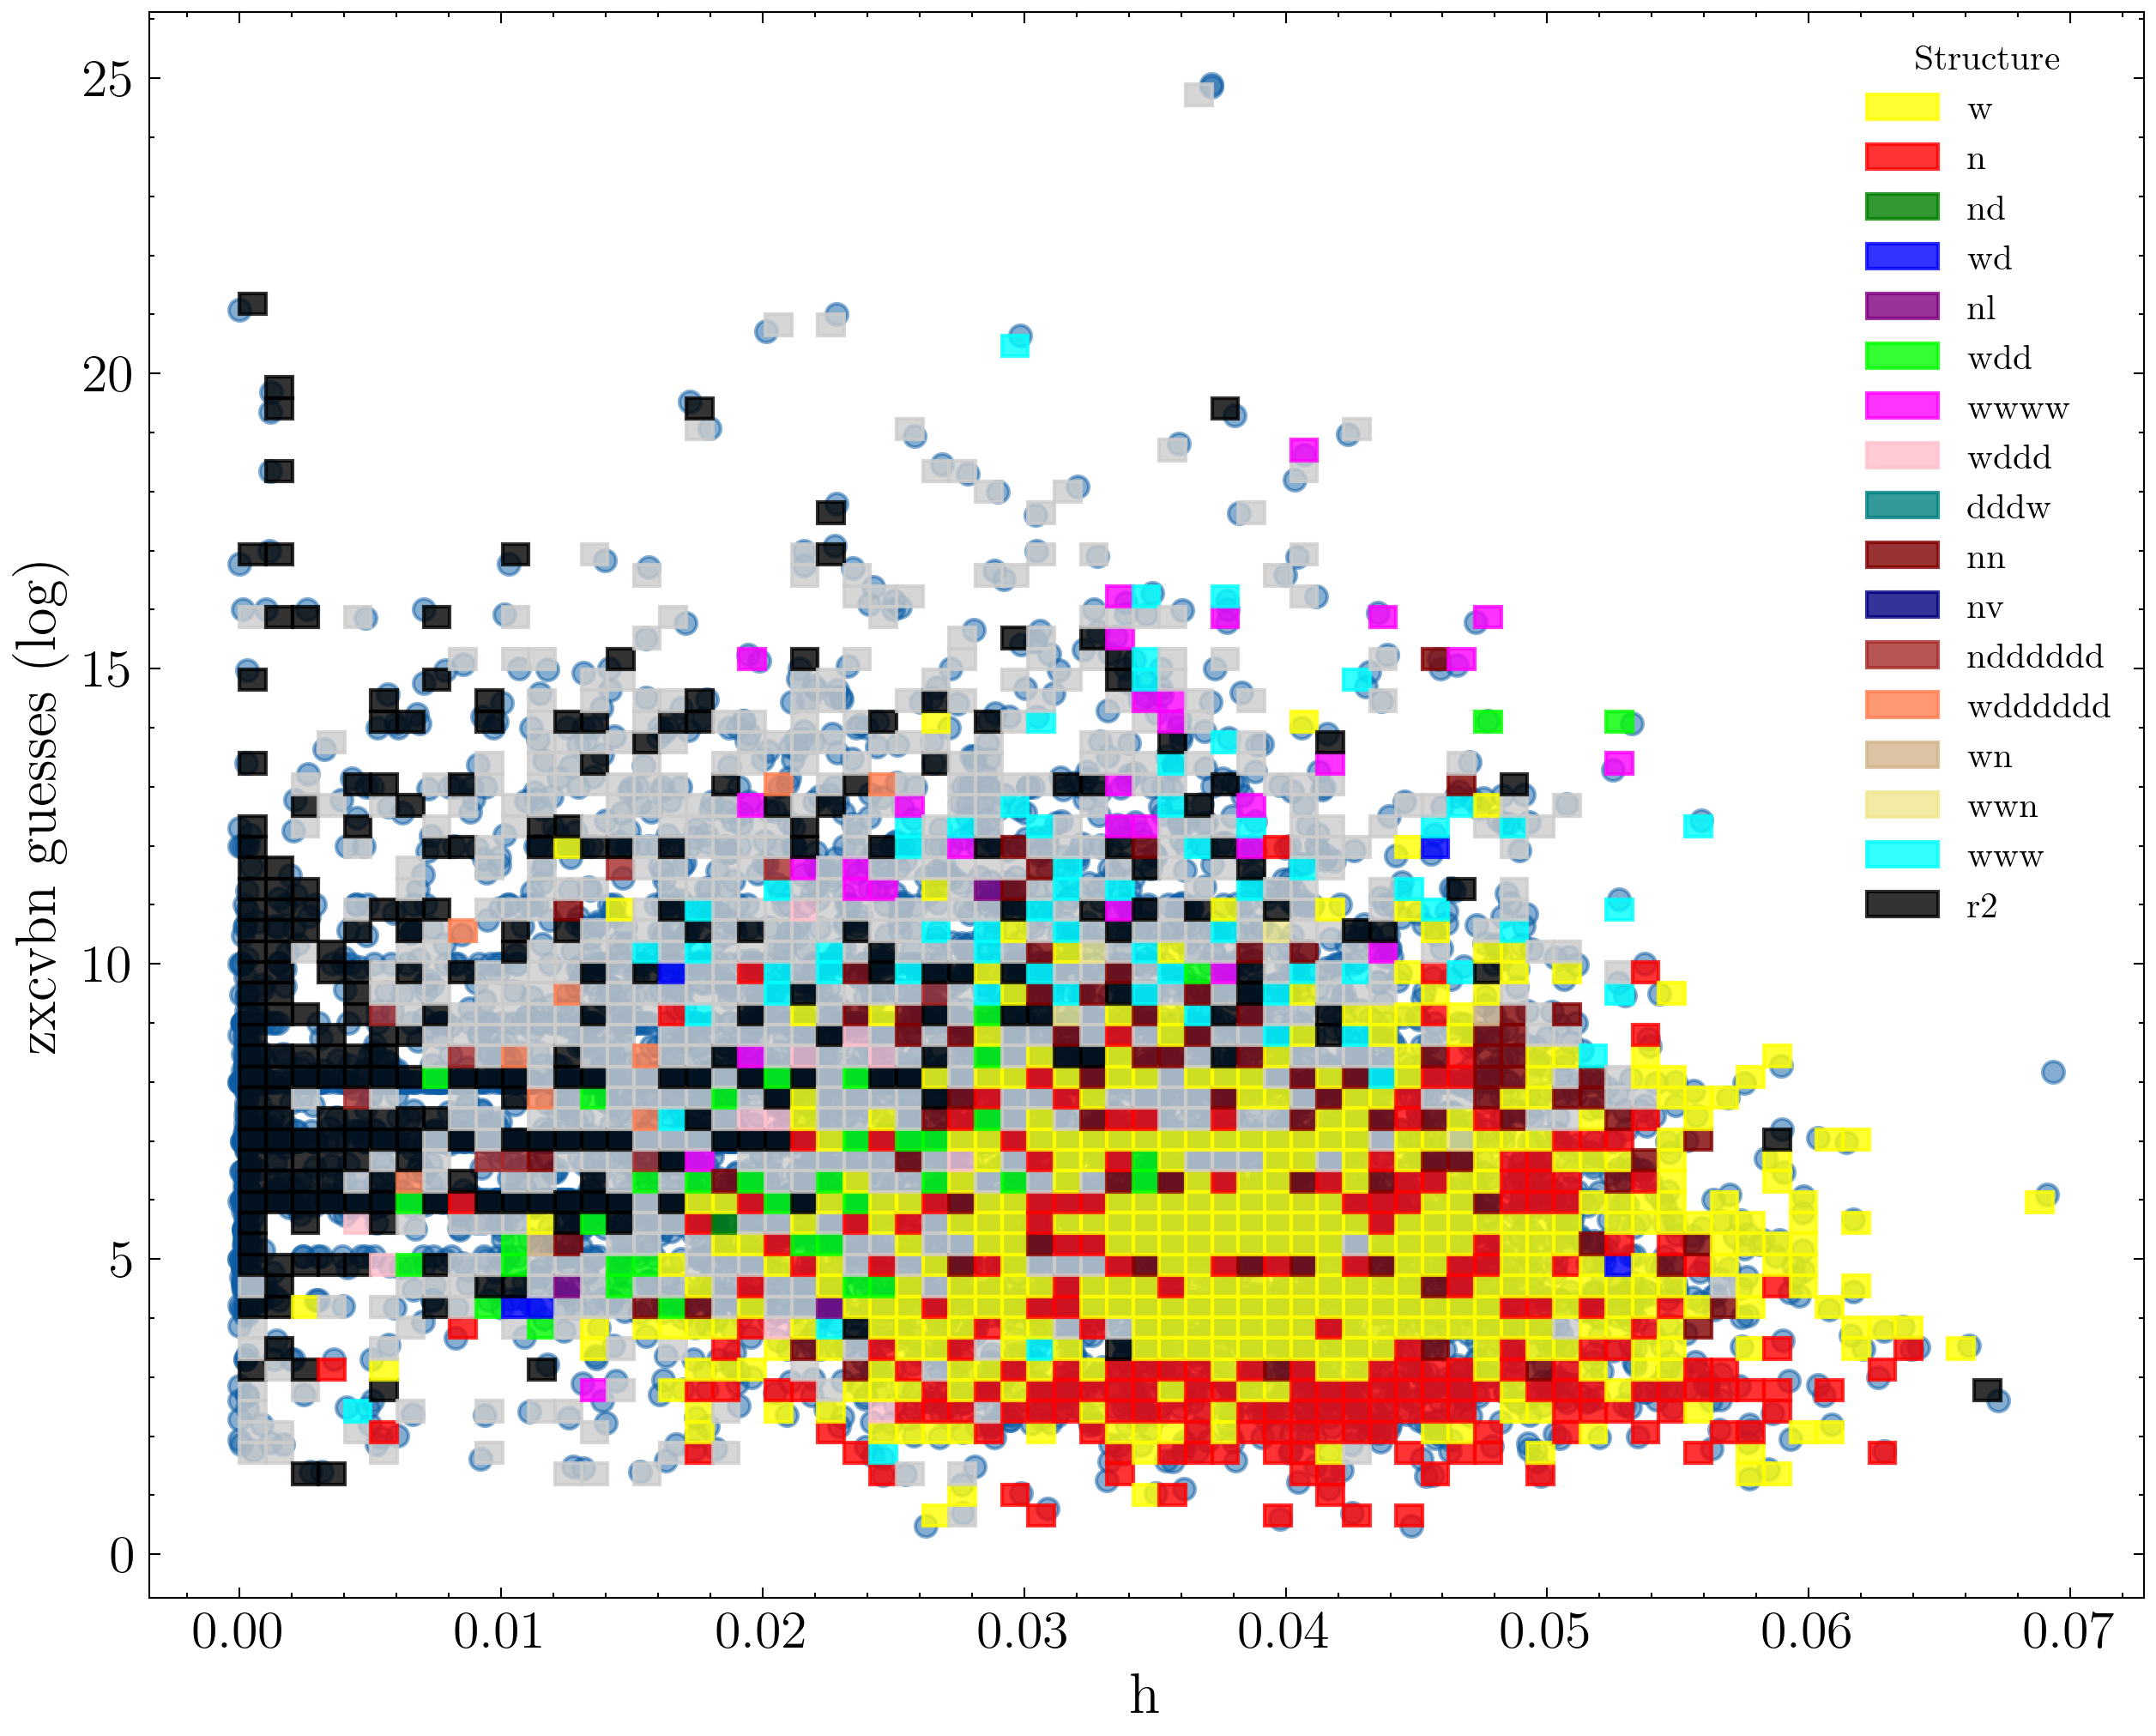
\includegraphics[scale=0.65]{figs/why_passwords/heatmap_structure.png}
        \caption{Chart showing the labelled \hmail passwords and their respective structure. Individual grids represent the most frequent structure. On the y axis we have the \zxcvbn \texttt{guesses\_log10} metric and on the x axis we have the $h$ = Markov 2-gram scores. As expected, the weakest passwords ($\bm{w}$: yellow and $\bm{n}$: red) have a high $h$ score and are predicted to be weak by \zxcvbnnocite. \srcOwnFig}
        \label{fig:heatmap_structure}
        %\vspace{-1em}
    \end{figure}
